% ETH Zurich  - 3D Photography 2015
% http://www.cvg.ethz.ch/teaching/3dphoto/
% Template for project proposals

\documentclass[11pt,a4paper,oneside,onecolumn]{IEEEtran}
\usepackage{graphicx}
% Enter the project title and your project supervisor here
\newcommand{\ProjectTitle}{3D Object Recognition with Deep Networks}
\newcommand{\ProjectSupervisor}{Martin Oswald, Pablo Speciale}
\newcommand{\DateOfReport}{March 7, 2015}

% Enter the team members' names and path to their photos. Comment / uncomment related definitions if the number of members are different than 2.
% Including photographs are optional. Photos are there to help us to evaluate your group more effectively. If you wish not to include your photos, please comment the following line.
\newcommand{\PutPhotos}{}
% Please include a clear photo of each member. (use pdf or png files for Latex to embed them in the document well)
\newcommand{\memberone}{Tobias Grundmann}
\newcommand{\memberonepicture}{pic1.png}
\newcommand{\membertwo}{Adrian Schneuwly}
\newcommand{\membertwopicture}{pic2.png}
\newcommand{\memberthree}{Johannes Oswald}
\newcommand{\memberthreepicture}{pic3.png}


%%%% DO NOT EDIT THE PART BELOW %%%%
\title{\ProjectTitle}
\author{3D Photography Project Proposal\\Supervised by: \ProjectSupervisor\\ \DateOfReport}
\begin{document}
\maketitle
\vspace{-1.5cm}\section*{Group Members}\vspace{0.3cm}
\begin{center}\begin{minipage}{\linewidth}\begin{center}
\begin{minipage}{3 cm}\begin{center}\memberone\ifdefined\PutPhotos\\\vspace{0.2cm}\includegraphics[height=3cm]{\memberonepicture}\fi\end{center}\end{minipage}
\ifdefined\membertwo\begin{minipage}{3 cm}\begin{center}\membertwo\ifdefined\PutPhotos\\\vspace{0.2cm}\includegraphics[height=3cm]{\membertwopicture}\fi\end{center}\end{minipage}\fi
\ifdefined\memberthree\begin{minipage}{3 cm}\begin{center}\memberthree\ifdefined\PutPhotos\\\vspace{0.2cm}\includegraphics[height=3cm]{\memberthreepicture}\fi\end{center}\end{minipage}\fi
\end{center}\end{minipage}\end{center}\vspace{0.3cm}
%%%% END OF PROTECTED LINES %%%%


%%%% BEGIN WRITING THE DOCUMENT HERE %%%%

\section{Description of the project}

 The main goal of our project is to enhance object recognition by making use of the recent availability of 2.5D  data through Microsoft Kinect, Google Project Tango, et al. 
We will follow recent approaches \cite{wu}, \cite{mat} which use convolutional deep neural/belief networks to learn the distribution of complex 3D shapes across different object categories of CAD models. Given 2.5D data of a single view point, we will try to recognise the objects category after an intense training of our deep network on a large scale 3D CAD model dataset. Fig. \ref{fig:idea}

\begin{figure}
  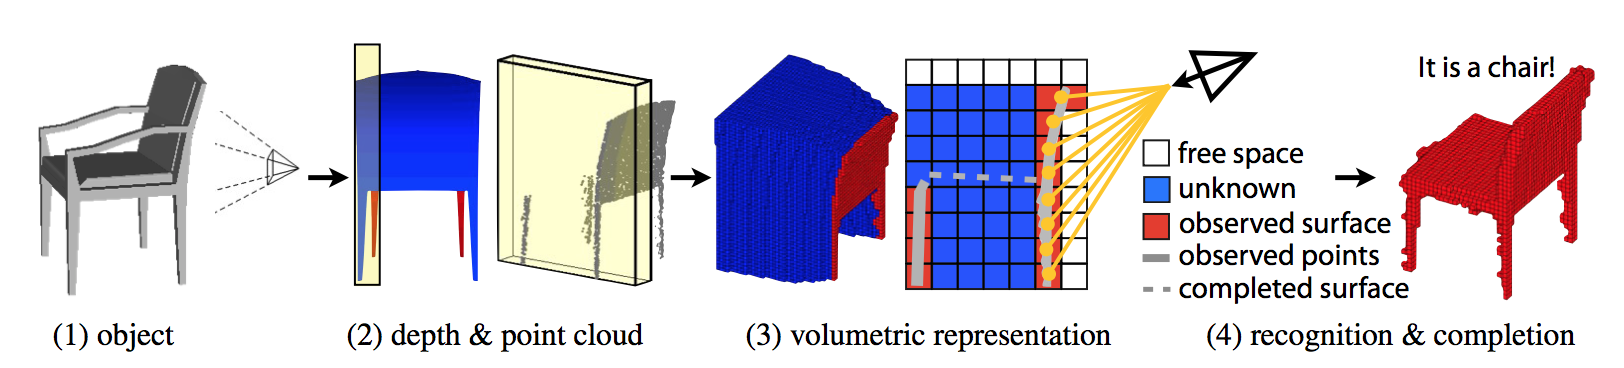
\includegraphics[width=\linewidth]{figure.jpg}
  \caption{}
  \label{fig:idea}
\end{figure}

\section{Work packages and timeline}

\subsection{Prerequisites in March}

The first goal of the team is to fully understand the approaches described in \cite{wu}, \cite{mat}. 
Therefore the team will work through the Udacity deep learning course \cite{uda} and extract knowledge and hands-on experience with deep networks for object recognition on 2D data.
At the end of the month, the team will be able to understand Deep Networks, its machine learning theory and TensorFlow (in Python) in order to develop a game plan for the project.
The division of work between the 3 project members will then be decided. 

\subsection{Data Preparation \& Modeling in April}
Deep Networks heavily depend on big datasets. Therefore we are going to use the ModelNet dataset from \cite{wu}, a CAD dataset of 660 objects. The datasets will transformed into 32x32x32 voxel data and split into a training, valuation and test set. If possible we will use data from the project tango tablet to cross test. We begin reimplementing the VoxNet Deep Convolutional Neural Network approaches in Python by starting with the deep learning udacity courses framework. \cite{uda} Therefore we will remodel the given 2D object recognition network into a rotation-invariant 3D recognition network which makes heavily use of convolution and pooling. The output of the deep network is the the class of object the network thinks it recognized from the input.

\subsection{Training \& Testing in June}
After successful implementation and testing, we will train the deep network on a subset of 40 classes called the ModelNet40 (optional: \cite{wu} offers an even larger data set) on own or universities GPU's.
Due to the computationally expensive training of the Deep Network on the large CAD dataset, we will try to start as soon as possible with this phase of the project.
\section{Outcomes and Demonstration}

Goal of the project is successfully reimplement the papers approaches for 3D Object Recognition and achieve very similar positive object recognition results. In our live demo, we will snapshot random CAD Models and try to recognise the object through our algorithm. 
 
\vspace{1cm}

{%\singlespace
{\small
\bibliography{refs}
\bibliographystyle{plain}}}




\end{document}
